% Graphic for TeX using PGF
% Title: /home/marta/Diagrama1.dia
% Creator: Dia v0.97.3
% CreationDate: Fri Sep  8 23:31:58 2017
% For: marta
% \usepackage{tikz}
% The following commands are not supported in PSTricks at present
% We define them conditionally, so when they are implemented,
% this pgf file will use them.
\ifx\du\undefined
  \newlength{\du}
\fi
\setlength{\du}{15\unitlength}
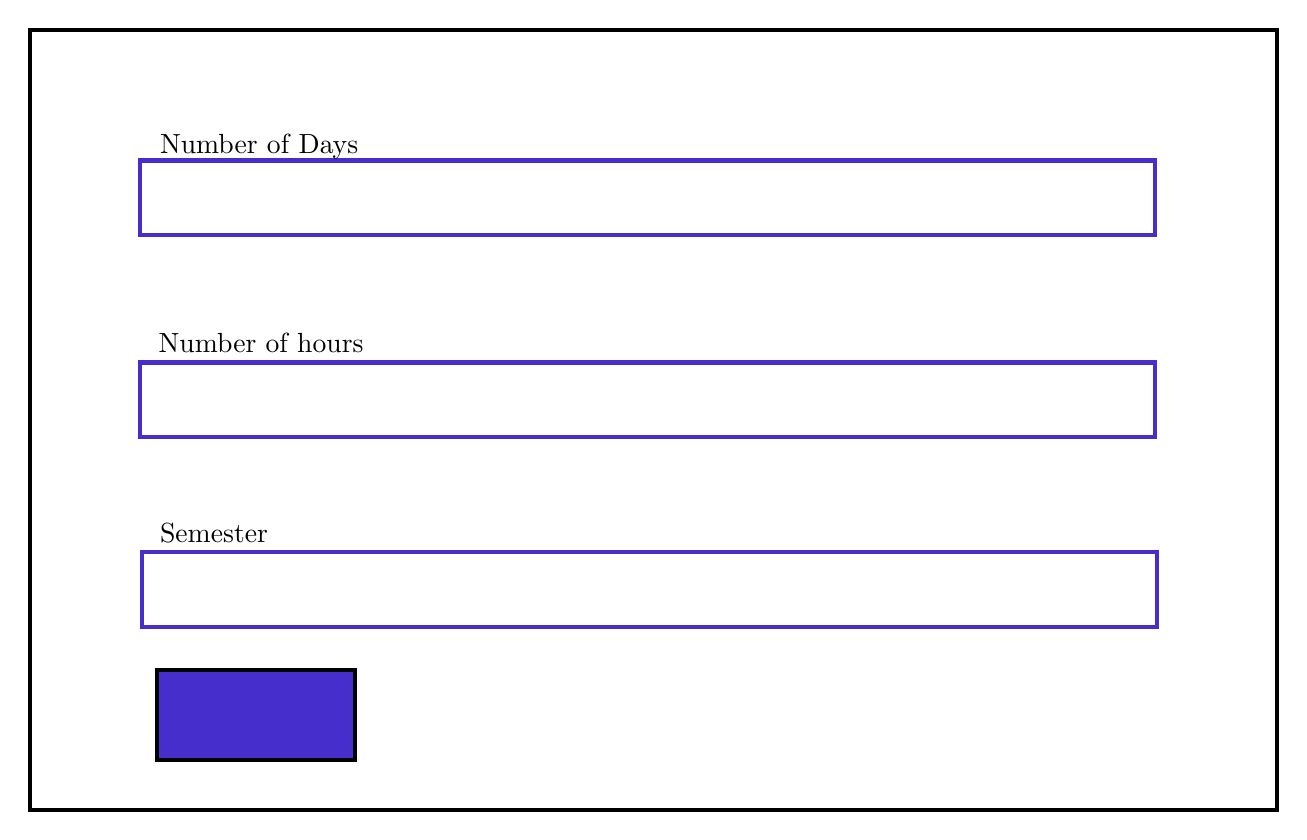
\begin{tikzpicture}
\pgftransformxscale{1.000000}
\pgftransformyscale{-1.000000}
\definecolor{dialinecolor}{rgb}{0.000000, 0.000000, 0.000000}
\pgfsetstrokecolor{dialinecolor}
\definecolor{dialinecolor}{rgb}{1.000000, 1.000000, 1.000000}
\pgfsetfillcolor{dialinecolor}
\pgfsetlinewidth{0.100000\du}
\pgfsetdash{}{0pt}
\pgfsetdash{}{0pt}
\pgfsetmiterjoin
\definecolor{dialinecolor}{rgb}{1.000000, 1.000000, 1.000000}
\pgfsetfillcolor{dialinecolor}
\fill (5.150000\du,4.950000\du)--(5.150000\du,23.750000\du)--(35.200000\du,23.750000\du)--(35.200000\du,4.950000\du)--cycle;
\definecolor{dialinecolor}{rgb}{0.000000, 0.000000, 0.000000}
\pgfsetstrokecolor{dialinecolor}
\draw (5.150000\du,4.950000\du)--(5.150000\du,23.750000\du)--(35.200000\du,23.750000\du)--(35.200000\du,4.950000\du)--cycle;
\pgfsetlinewidth{0.100000\du}
\pgfsetdash{}{0pt}
\pgfsetdash{}{0pt}
\pgfsetmiterjoin
\definecolor{dialinecolor}{rgb}{1.000000, 1.000000, 1.000000}
\pgfsetfillcolor{dialinecolor}
\fill (7.800000\du,8.100000\du)--(7.800000\du,9.900000\du)--(32.250000\du,9.900000\du)--(32.250000\du,8.100000\du)--cycle;
\definecolor{dialinecolor}{rgb}{0.270588, 0.180392, 0.800000}
\pgfsetstrokecolor{dialinecolor}
\draw (7.800000\du,8.100000\du)--(7.800000\du,9.900000\du)--(32.250000\du,9.900000\du)--(32.250000\du,8.100000\du)--cycle;
\pgfsetlinewidth{0.100000\du}
\pgfsetdash{}{0pt}
\pgfsetdash{}{0pt}
\pgfsetmiterjoin
\definecolor{dialinecolor}{rgb}{1.000000, 1.000000, 1.000000}
\pgfsetfillcolor{dialinecolor}
\fill (7.810375\du,12.965000\du)--(7.810375\du,14.765000\du)--(32.260375\du,14.765000\du)--(32.260375\du,12.965000\du)--cycle;
\definecolor{dialinecolor}{rgb}{0.270588, 0.180392, 0.800000}
\pgfsetstrokecolor{dialinecolor}
\draw (7.810375\du,12.965000\du)--(7.810375\du,14.765000\du)--(32.260375\du,14.765000\du)--(32.260375\du,12.965000\du)--cycle;
\pgfsetlinewidth{0.100000\du}
\pgfsetdash{}{0pt}
\pgfsetdash{}{0pt}
\pgfsetmiterjoin
\definecolor{dialinecolor}{rgb}{1.000000, 1.000000, 1.000000}
\pgfsetfillcolor{dialinecolor}
\fill (7.858300\du,17.530000\du)--(7.858300\du,19.330000\du)--(32.308300\du,19.330000\du)--(32.308300\du,17.530000\du)--cycle;
\definecolor{dialinecolor}{rgb}{0.270588, 0.180392, 0.800000}
\pgfsetstrokecolor{dialinecolor}
\draw (7.858300\du,17.530000\du)--(7.858300\du,19.330000\du)--(32.308300\du,19.330000\du)--(32.308300\du,17.530000\du)--cycle;
\pgfsetlinewidth{0.100000\du}
\pgfsetdash{}{0pt}
\pgfsetdash{}{0pt}
\pgfsetmiterjoin
\definecolor{dialinecolor}{rgb}{0.270588, 0.180392, 0.800000}
\pgfsetfillcolor{dialinecolor}
\fill (8.221807\du,20.371157\du)--(8.221807\du,22.543358\du)--(12.987683\du,22.543358\du)--(12.987683\du,20.371157\du)--cycle;
\definecolor{dialinecolor}{rgb}{0.000000, 0.000000, 0.000000}
\pgfsetstrokecolor{dialinecolor}
\draw (8.221807\du,20.371157\du)--(8.221807\du,22.543358\du)--(12.987683\du,22.543358\du)--(12.987683\du,20.371157\du)--cycle;
% setfont left to latex
\definecolor{dialinecolor}{rgb}{0.000000, 0.000000, 0.000000}
\pgfsetstrokecolor{dialinecolor}
\node[anchor=west] at (7.984733\du,12.502007\du){Number of hours};
% setfont left to latex
\definecolor{dialinecolor}{rgb}{0.000000, 0.000000, 0.000000}
\pgfsetstrokecolor{dialinecolor}
\node[anchor=west] at (8.017154\du,7.768553\du){Number of Days};
% setfont left to latex
\definecolor{dialinecolor}{rgb}{0.000000, 0.000000, 0.000000}
\pgfsetstrokecolor{dialinecolor}
\node[anchor=west] at (8.017154\du,17.073358\du){Semester};
\end{tikzpicture}
